\documentclass[titlepage]{article}
\usepackage[a4paper,margin=0.7in]{geometry}
\usepackage{rotating}
\usepackage{pgfgantt}
\usepackage{pgfcalendar}
\usepackage{datetime}
\usepackage[none]{hyphenat}

\usepackage{relsize}

\usepackage{tikz}
\usetikzlibrary{calc,shapes,chains,scopes,shapes.multipart}

\usepackage{forest}
\forestset{}

\pagenumbering{gobble}
\setganttlinklabel{f-s}{}
\setganttlinklabel{s-s}{}
\setganttlinklabel{f-f}{}
% Begin new command
\title{Tutorial 1-1: Project Management}
\author{
	Group D1:\\\\\\
	Aliia Almazbekova - 24346158\\\\
	Jasper Chan - 37467164\\\\
	Jacky Chan - 19835164\\\\
	Matteo Ferraresso - 36470169\\\\
	Adrian Lam - 23735160\\\\
	Janelle Lawson - 34680165\\\\
	David Stewart - 54071155\\\\
}
%\for{MECH 223 Instructors, University of British Columbia}

\begin{document}

\maketitle


\begin{sidewaysfigure}
	\centering
	\noindent\resizebox{\textwidth}{!}{
		\begin{ganttchart}[
		x unit=0.45cm,
		y unit chart=0.6cm,
		hgrid,vgrid={dotted},
			bar label node/.style={text width=1.5in, align=right,anchor=east,font=\relsize{-2}},
			group label node/.style={text width=1.5in, align=right,font=\bf\relsize{-2},anchor=east},
			milestone label node/.style={text width=1.5in, align=right,font=\em\relsize{-2},anchor=east},
        ]
		{04}{29}
			\newcommand{\barcolor}[1]{{bar/.style={fill=#1}}}
			\newcommand{\groupcolor}[1]{group/.append style={fill=#1}}
			\gantttitlelist{4,...,29}{1} \\
			
			\ganttbar{Project Management Meeting}{4}{4}\\
			\ganttbar[name=congen]{Concept Generation}{7}{8}\\

			\ganttgroup[name=eval, group/.append style={fill=red}]{Evaluation}{9}{11}\\
			\ganttbar[name=winnow, bar/.append style={fill=red}]{Winnowing}{9}{9}\\
			\ganttbar[name=rank, bar/.append style={fill=red}]{Ranking}{9}{9}\\
			\ganttbar[name=score, bar/.append style={fill=red}]{Scoring}{10}{11}\\
			\ganttlink[link type=f-s]{winnow}{rank}
			\ganttlink{rank}{score}
%			\ganttlink{congen}{eval}
			\ganttlink[link type=f-s]{congen}{winnow}

			\ganttgroup[name=design, group/.append style={fill=blue}]{Detailed Design}{12}{18}\\
			\ganttbar[name=build, bar/.append style={fill=blue}]{Building}{12}{18}\\
			\ganttbar[name=test, bar/.append style={fill=blue}]{Testing}{12}{18}\\
%			\ganttlink{score}{design}
			\ganttlink[link type=f-s]{score}{build}
			\ganttlink[link type=f-s]{score}{test}

			\ganttmilestone{Preliminary prototype}{12} \\

			\ganttgroup[group/.append style={fill=green}]{Report}{8}{29}\\
			\ganttbar[bar/.append style={fill=green}]{Body}{8}{20}\\
			\ganttbar[bar/.append style={fill=green}]{Editing}{21}{29}\\

			\ganttbar[name=poster]{Poster}{19}{24}\\
			\ganttbar[name=presentation]{Presentation}{19}{26}\\
			\ganttmilestone[name=poscom]{Poster \& Competition Due}{24}\\
			\ganttbar[name=rec,bar/.append style={fill=green}]{Conclusion and Recommendation}{25}{29}\\
			\ganttlink{poster}{poscom}
			\ganttlink{design}{poscom}
			\ganttlink{build}{poscom}
			\ganttlink{test}{poscom}
			\ganttlink{poscom}{rec}

			\ganttmilestone[name=present]{Presentation}{26}
			
			\ganttlink{presentation}{present}

		\end{ganttchart}
	}
\end{sidewaysfigure}

\def\time{\nodepart{two}}

\begin {sidewaysfigure}[h]
	\centering
	\noindent\resizebox{\textwidth}{!}{
		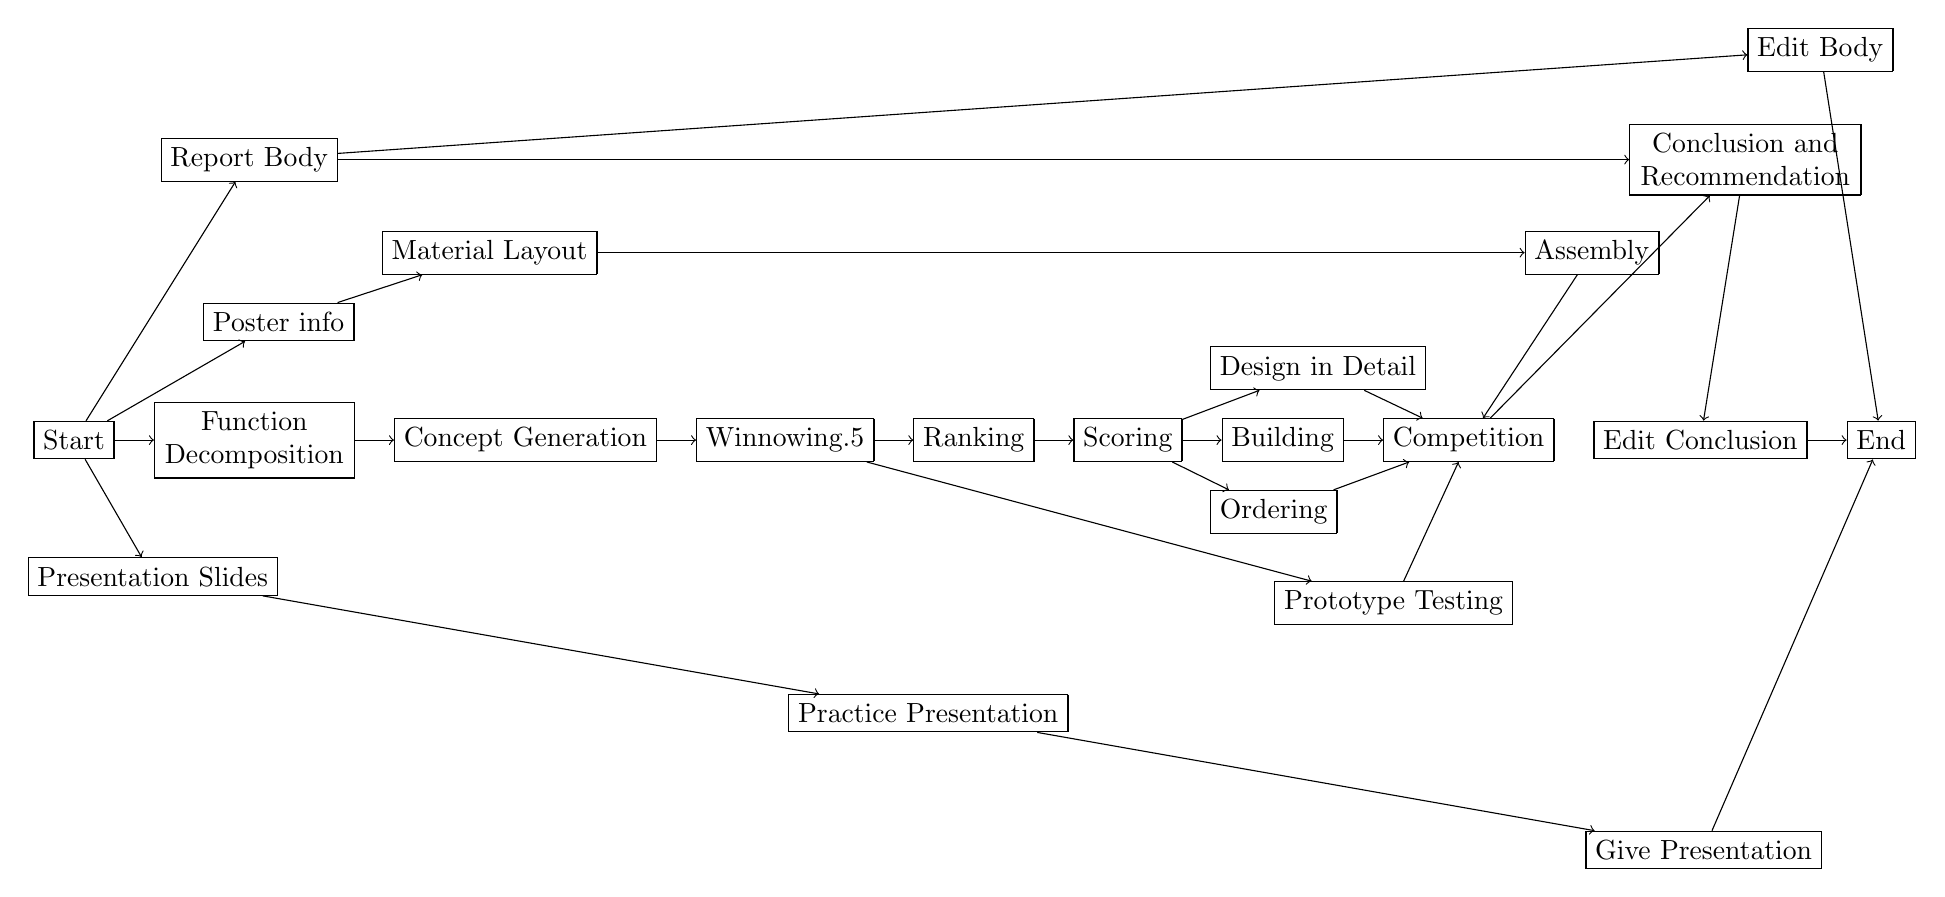
\begin{tikzpicture}[
			node distance=5mm, 
			every on chain/.style={
				join,
				rectangle split,
				rectangle split horizontal,
				rectangle split parts=2,
				rectangle split ignore empty parts,
				align=center,
				draw,
			}, 
			every join/.style={->},
		]
		{
			[start chain=main]
			\node (start) [on chain] {Start};
			{ [start branch=report]
				\node (reportbody) [on chain=going {at=(\tikzchainprevious),shift=(58:2.1)}] {Report Body\time7};
				{ [start branch=editbody]
					\node (editbody) [on chain=going {at=(\tikzchainprevious),shift=(4:10)}] {Edit Body\time4};
				}
			}
			{ [start branch=poster]
				\node (posterinfo) [on chain=going {at=(\tikzchainprevious),shift=(30:1.5)}] {Poster info\time3};
				\node (materiallayout) [on chain=going above right] {Material Layout\time1};
				\node (assembly) [on chain=going {at=(\tikzchainprevious),shift=(0:7)}] {Assembly\time1};
			}
			{ [start branch=presentation]
				\node [on chain=going {at=(\tikzchainprevious),shift=(-60:1)}] {Presentation Slides\time5};
				\node [on chain=going {at=(\tikzchainprevious),shift=(-10:5)}] {Practice Presentation\time2};
				\node [on chain=going {at=(\tikzchainprevious),shift=(-10:5)}] {Give Presentation\time1};
			}
			\node (functiondecomp) [on chain] {\nodepart[text width=2.3cm]{one}Function Decomposition\time1};
			\node (conceptgeneration) [on chain] {Concept Generation\time2};
			\node (winnowing) [on chain] {Winnowing\time0.5};
			{ [start branch=prototype]
				\node (prototypetesting) [on chain=going {at=(\tikzchainprevious), shift=(-15:4)}] {Prototype Testing\time3};
			}
			\node [on chain] {Ranking\time1};
			\node (scoring) [on chain] {Scoring\time2};
			{ [start branch=design]
				\node [on chain=going above right] {Design in Detail\time9};
			}
			{ [start branch=ordering]
				\node [on chain=going below right] {Ordering\time6};
			}
			\node (building) [on chain] {Building\time10};
			\node (competition) [
				on chain,
				join=with main/design-end, 
				join=with main/ordering-end,
				join=with main/poster-end,
				join=with main/prototype-end,
			] {Competition\time1};
			{ [continue branch=report]
				\node (conclusion) [on chain=going {at=(\tikzchainprevious), shift=(0:9.5)},join=with competition] {\nodepart[text width=2.7cm]{one} Conclusion and Recommendation\time2};
				%\node (editconclusion) [on chain=going {at=(\tikzchainprevious),shift=(-55:1.5)}] {Edit Conclusion\time2};
				\node (editconclusion) [on chain, right=of competition] {Edit Conclusion\time2};
				\node (end) [
					on chain,
					join=with main/presentation-end,
					join=with main/report/editbody-end,
				] {End};
			}
		}
		\end{tikzpicture}
	}
\end{sidewaysfigure}

\end{document}

